%%%%%%%%%%%%%%%%%%%%%%%%%%%%%%%%%%%%%%%%%%%%%%%%%%%%%%%%%%%%%%%%%%%%%%
%%                     Unit of Information
%%%%%%%%%%%%%%%%%%%%%%%%%%%%%%%%%%%%%%%%%%%%%%%%%%%%%%%%%%%%%%%%%%%%%%
%\color{blue}

\subsection{Glyph: \glyph{Unit of information}}
\label{sec:unitInformation}

When representing biological entities, it is often necessary to convey some abstract information about the entity's function or structure.  The SBGN \glyph{unit of information} is a decoration that can be used in this situation to add information to a glyph.  Some example uses of a \glyph{unit of information} include (but are not limited to) specifying is an interaction is intra or intermolecular, information about the physical environment, or the specific type of biological entity it is decorating.

\begin{glyphDescription}

\glyphSboTerm Not applicable.

\glyphContainer A unit of information is represented by a rectangle.  The long side of the rectangle should be oriented parallel to the border of the \glyph{entity}, or the edge, being annotated by the \glyph{unit of information}. The center of the bounding box of a \glyph{unit of information} should be located on the mid-line of the border of the carrying \glyph{entity} or the carrying edge.

\glyphLabel A \glyph{unit of information} is identified by a label placed in an unbordered box containing a string of characters.  The characters can be distributed on several lines to improve readability, although this is not mandatory.  The label box must be attached to the center of the container.  The label may spill outside of the container.

The label defines the information carried by the \glyph{unit of information}.  \SBGNERLone defines several reserved labels, such as ``cis'' and ``trans'', or specific prefixes that must be included in the label to indicate the type of information (\sect{CVs}).

\glyphAux A \glyph{unit of information} does not carry any auxiliary items.

\end{glyphDescription}

\begin{figure}[H]
  \centering
  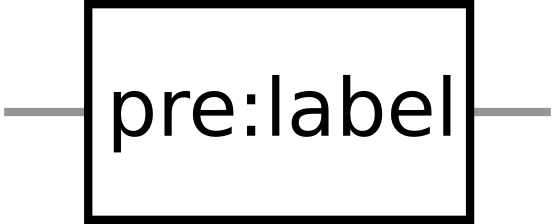
\includegraphics[scale = 0.3]{images/unitInformation}
  \caption{The \ER glyph for \glyph{unit of information}.}
  \label{fig:unitInformation}
\end{figure}


\begin{figure}[H]
  \centering
  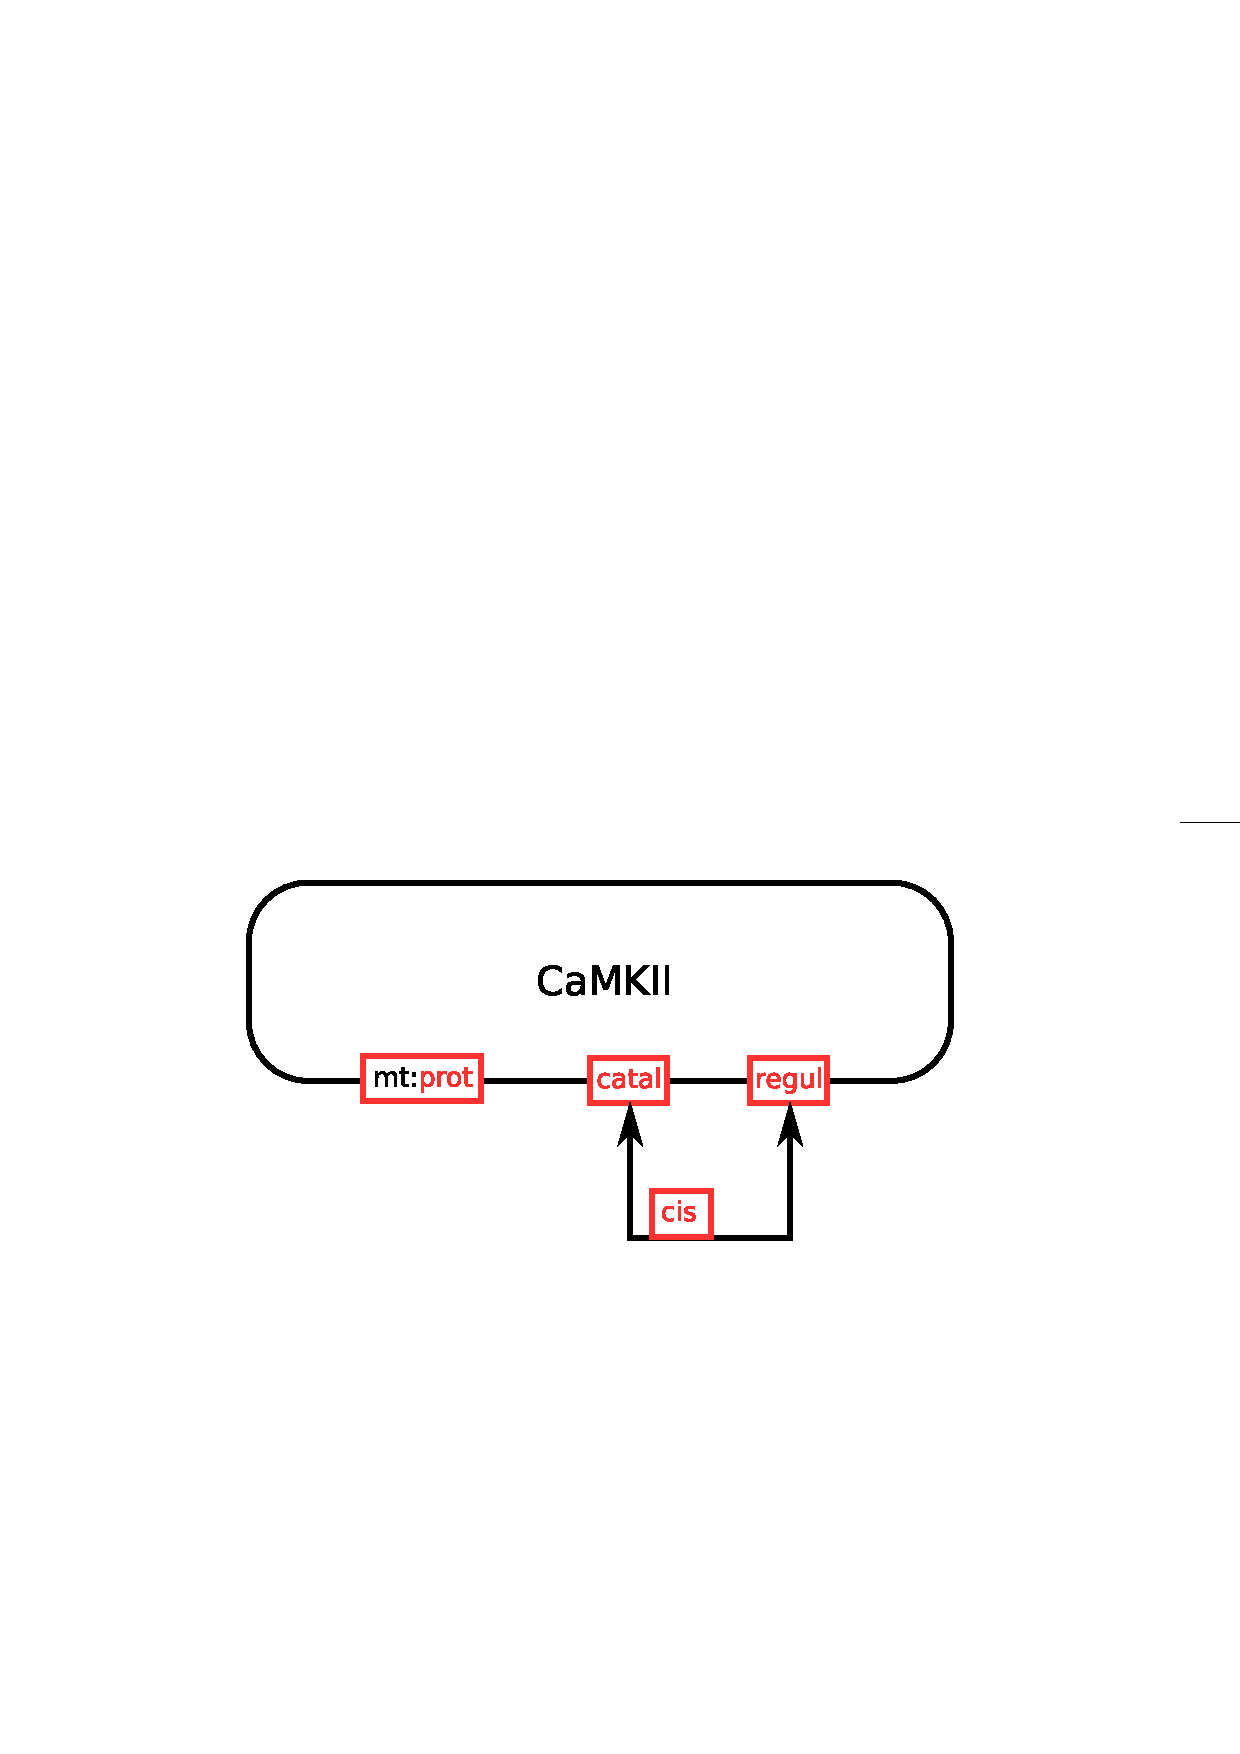
\includegraphics[scale = 0.5]{examples/ex-unitInformation}
  \caption{Using \glyph{units of information} to represent the fact that the entity ``CaMKII'' is a protein, and can display intra- (cis) and inter- (trans) molecular interactions.}
  \label{fig:ex-unitInformation}
\end{figure}

%\normalcolor
